\documentclass{article}
\usepackage[margin=1in]{geometry}
\usepackage{../common}
\usepackage{../pagesetup}
\usepackage{float}
% **** IF YOU WANT TO DEFINE ADDITIONAL MACROS FOR YOURSELF, PUT THEM HERE:

\def\mathrlap{\mathpalette\mathrlapinternal} 
\def\mathclap{\mathpalette\mathclapinternal}
\def\mathllapinternal#1#2{\llap{$\mathsurround=0pt#1{#2}$}}
\def\mathrlapinternal#1#2{\rlap{$\mathsurround=0pt#1{#2}$}}

\begin{document}


\lecture{14}{October 25}{Sasha Rush}{Eric Dunipace, Andrew Fai, Isaac Xia}{Mixture Models}


\subsection{Administrative Announcements}

Overview:  Second half of class is on Inference, especially on harder problems.  There is only one problem set left, but the bulk of the time will be on the project.

There is some extra time left in the schedule, for which Prof. Rush will poll topics from the class.

\subsection{Mixture Models: Introduction}

Up until now, we've been considering mostly supervised learning, where we had an input $x$, an output $y$, and parameters $\theta$.

Previously when doing MLE, MAP, marginalizing over nodes in a graphical model, we weren't trying to find a distribution, we were finding a {\bf point-estimation} rather than a {\bf distribution}.

For example, suppose we want to think about models from Naive Bayes:


\begin{center}
\begin{tikzpicture}
  %Define nodes
  \node[latent] (y) {$y_n$};
  \node[latent, above=of y] (pi) {$\pi$};
  \node[latent, below=of y, xshift=-1cm]  (x1) {$x_{1,n}$};
  \node[latent, below=of y, xshift=1cm]  (xv) {$x_{V,n}$};
  \node[latent, below=of x1, xshift = 1cm] (mu) {$\mu_k$};

  % Connect the nodes
  \edge {y} {x1};
  \edge {y} {xv};
  \edge {pi} {y};
  \edge {mu} {x1};
  \edge {mu} {xv};
  
  \path (x1) -- node[auto=false]{\ldots} (xv);
    \plate {plate} {(y)(x1)(xv)} {$n$} ;
    \plate {plate} {(mu)} {$k$}
\end{tikzpicture}
\end{center}

with joint probability $$\displaystyle p(y | \pi) \prod_{j= 1}^V p(x_j | y, \mu),$$ where the priors could be Categorical on $p(y | \pi)$ and Bernoulli on each $p(x_j | y, \mu)$.  

In this setting, with data $\{x_i, y_i\}$, we can perform log-likelihood maximization with $p(\{x\}, \{y\})$ to infer the parameters $\mu$ and $\pi$.

\smallskip

In a new setting, instead suppose we have the same graphical plate model, but we now do not observe the categories; instead of $y_n$, we denote these latent variables as $z_n$.

\begin{center}
\begin{tikzpicture}
  %Define nodes
  \node[latent] (z) {$z_n$};
  \node[latent, above=of z] (pi) {$\pi$};
  \node[latent, below=of z, xshift=-1cm]  (x1) {$x_{1,n}$};
  \node[latent, below=of z, xshift=1cm]  (xv) {$x_{V,n}$};
  \node[latent, below=of x1, xshift = 1cm] (mu) {$\mu_k$};

  % Connect the nodes
  \edge {z} {x1};
  \edge {z} {xv};
  \edge {pi} {z};
  \edge {mu} {x1};
  \edge {mu} {xv};
  
  \path (x1) -- node[auto=false]{\ldots} (xv);
	\plate {plate} {(z)(x1)(xv)} {$n$} ;
	\plate {plate} {(mu)} {$k$}

\end{tikzpicture}
\end{center}
which also can be represented with the following undirected graphical model:
\begin{center}
	\begin{tikzpicture}[]
	
	%Define nodes
	\node[latent] (z) {$z_n$};
	\node[latent, above=of z] (pi) {$\pi$};
	\node[latent, below=of z, xshift=-1cm]  (x1) {$x_{1,n}$};
	\node[latent, below=of z, xshift=1cm]  (xv) {$x_{V,n}$};
	\node[latent, below=of x1, xshift = 1cm] (mu) {$\mu_k$};
	
	% Connect the nodes
	\path[draw]
	(z) edge node {}  (x1)
	(z) edge node {}  (xv)
	(z) edge node {}  (mu)
	(pi) edge node {}  (z)
	(mu) edge node {}  (x1)
	(mu) edge node {}  (xv);
	
	
	\path (x1) -- node[auto=false]{\ldots} (xv);
	\plate {plate} {(z)(x1)(xv)} {$n$} ;
	\plate {plate} {(mu)} {$k$}
	
	\end{tikzpicture}
\end{center}

What does this graphical model look like, and what dependencies do we need to consider?  

\begin{itemize}
	\item There's clearly a dependency on $\pi$, but we can't observe $z_n$.
	\item There are the $\mu_k$ from the $x_{in}$.
\end{itemize}


All of these Naive Bayes models without observed $y_n$ are used for {\bf different types of clustering}. These models are referred to as {\bf mixture models}, and can handle  multimodality well.  

\subsection{Types of Mixture Models}
Up until now, most models we've used have unimodal distributions, e.g. normal distributions.

\begin{figure}[H]
\begin{center}
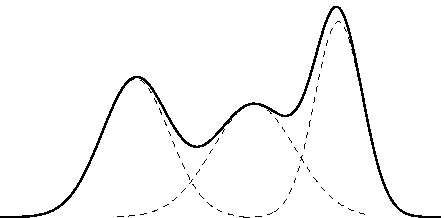
\includegraphics[scale=0.5]{multimodal.jpg}
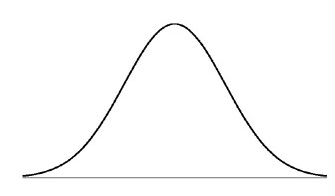
\includegraphics[scale=0.5]{gaussian.jpg}
\caption{Multimodality of Multiple Gaussians vs Unimodality of One Gaussian}
\end{center}
\end{figure}   

Although we won't limit ourselves to only using continuous mixture models, we'll be primarily working with mixtures of Gaussians.  Below are examples of mixture models we'll see more of.

\subsubsection{Mixture of Gaussian Modes}
	We can have a mixture of Gaussian models, by simply mixing different Gaussian conditional distributions together:

	\[p(x | y) \sim \mathcal{N}(\mu, \Sigma)  \]

	An application example is speech recognition, which must deal with different accents (e.g. British vs American) for pronunciations of the same word.  In this case, Gaussian mixture models are able to consolidate the seemingly different pronunciations.


\subsubsection{Mixture of Bernoulli/Multinomial Models}

	We can instead mix together various Bernoulli or Multinomial conditionals. 

	\[ p(x_j | y) \sim \on{Bern}(\mu_j) \text{ or } \on{Multinom}(\alpha) \]

	% [Diagram of sports/politics/school?]

	% [Commentary on applications?]

%%%%%%%%%%%%%%%%%%%%%%%%%%%%%%%% 
\subsection{Math behind Mixture Models}

Now, we delve more deeply into the math behind using such mixture models.  To start, the models involve $x$ (data), $z$ (latent variables), $\pi$ (prior of latent variable), and $\{\mu_k\}$ (parameters for conditional distribution).  We will use $x$ and $z$ to denote all $n$ observations of the data and latent variables.

\smallskip

The {\bf complete data likelihood} of the model is then 
\[ p(x, z) = \prod_{n} \prod_{k} \pi_k p(x_n | \mu_k)^{z_{nk}},  \]
where $z_{nk}$ is shorthand for $\mathbf{1}(Z_n = k)$.

To get the {\bf marginal likelihood} of the data, we can marginalize and sum over all possible values of $z_n$:	

\[p(x) = \sum_{z} \prod_n \prod_k \pi_k p(x_n | \mu_k)^{{z_{nk}}} = \prod_n \underbrace{\sum_{z}}_{\text{Hard to compute}} \prod_k \pi_k p(x_n | \mu_k)^{z_{nk}}  \]

Although we pushed the sum into the product, the sum over all possible values of $z$ is still hard to compute.  Our main alternative strategy is thus to utilize the complete data likelihood in order to find $p(x)$.  

Below is a heuristic algorithm to find $p(x)$:
\begin{enumerate}
	\item Initialize $\pi$ and $\mu$ randomly.
	\item Compute the log-likelihood $\displaystyle p(x, z | \pi, \mu) = \sum_n \sum_k z_{nk} \log \pi_k + z_{nk} \log p(x_n |\mu_k)$ using fixed $\pi$ and $\mu$.
	\item Denote $q_{nk} = p(z_n = k | x_n ;... )$ as a ``hallucinated'' distribution over $z_{nk}$; the origin of $q_{nk}$ is unclear, but it satisfies the given requirements.  We can use this distribution of $z \sim q_{nk}$ to compute the expectation of the log-likelihood as:

	\begin{align*}
	\E_{z \sim q_{nk}} \left[ \log p(x_n, z_n | \pi, \mu) \right]	&= \sum_n \sum_k q_{nk} \log \pi_k + q_{nk} \log p(x_n | \mu_k).
	\end{align*}

	We can then ``hallucinate'' parameters through the distribution of $z_{nk}$!  Returning to the graphical model, recall that it was difficult to actually compute the parameters.  Howevere, given some parameters $\pi,\mu$, we can compute a marginal distribution over the $z$: $p(z | x, \pi, \mu)$.

	\item We thus can perform a coordinate ascent algorithm; that is, we optimize one set of parameters, then the other, then continue to alternate optimization.
\end{enumerate}

This heuristic is summarized below:

\begin{algorithm}
\begin{algorithmic}[1]
  \Procedure{EM\_NB}{$x,z$}
  \State{Initialize $\pi$ and $\mu$ randomly.}
  \While{$\pi$ and $\mu$ not converged}
  \State{(\emph{Expectation}) Compute $q_{nk} = p(z | x, \pi, \mu)$ using fixed $\pi$ and $\mu$}
  \State{(\emph{Maximization}) Compute MLE of $\pi$ and $\mu$ using $q$ through $\displaystyle \mathbb{E}_{z \sim q}\left[\log p(x ,z) \right]$}
  \EndWhile{}
  \EndProcedure{}
\end{algorithmic}
\end{algorithm}


The above is called the {\bf Expectation Maximization} (EM) Algorithm, where step 4 computes the actual expectation maximization, and step 5 actually maximizes through the MLE.  $\pi$ will be Categorical and $\mu$ will be the means of the Gaussians themselves here.

\subsection{Expectation Maximization Algorithm}

The above algorithm can be generalized, and is known as the {\bf Expectation Maximization} (EM) algorithm.



\begin{algorithm}[H]
\begin{algorithmic}[1]
  \Procedure{EM}{$x$,$z$}
  \State{Initialize $\pi$ and $\mu$ randomly.}
  \While{$\pi$ and $\mu$ not converged}
  \State{(\emph{Expectation}) $\displaystyle q_{nk} \gets \frac{\pi_k p(x_n | \mu_c)}{\sum\limits_{k'} \pi_{k'} p(x_n | \mu_{k'})}$}
  \State{(\emph{Maximization}) $\displaystyle \mathbb{E}_{z \sim q} \left[\log p(x, z| \pi, \mu) \right] = \sum_n \sum_k q_{nk} \log \pi_k + q_{nk} \log p(x_n | \mu_k)$}
  \EndWhile{}
  \EndProcedure{}
\end{algorithmic}
\end{algorithm}


We'll thinking about this algorithm in the context of information theory.  In the \emph{maximization} step, we have the first term $\displaystyle \sum_n \sum_k q_{nk} \log \pi_k$ can be thought about as maximizing the $\pi_k$ under the model, with the assumption they were sampled from distribution of $q_{nk}$. 

\[\sum_n \sum_k \underbrace{{q_{nk}}}_{\text{Came from $q_{nk}$ guess}} \log \left(\underbrace{{\pi_k}}_{\text{Want to find $\pi_k$}}\right) \]

So, we can think of $q_{nk}$ as ``expected counts'' from a distribution.  So, the MLE is similar to standard counts of observations.  In particular,
\[ \pi_k = \frac{\sum\limits_n q_{nk}}{\sum\limits_{n, k} q_{nk}}. \]

Alternatively, we could also use the MAP estimate.  The main point is that the prior is embedded in the max step.

A similar update happens for $\mu$, but will be specific to the actual form of the model $p(x | \mu)$.

\subsubsection{Assumptions on EM}

One key point is that the model yields an easily computable $p(z | x, \pi, \mu)$.  If we imagine that $p(x|z)$ is an arbitrary neural net with continuous output, this could be very difficult.  A specific example is a Variational Autoencoder (VAE), which could be found from Kingsma and Welling.


\subsection{Demo on EM}

We did a demonstration on Expectation Maximization.

In general, we saw it was pretty hard to even infer the clusters of data especially as the number of true clusters increased. 

{\bf Q:} \emph{How to infer number of true clusters?}  It's actually a hard problem, no really good standout way to do this.

{\bf Q:} \emph{Difference between $k$-means and EM here?}  $k$-means will choose $q$ as the highest probability, instead of assigning a distribution to $q_{nk}$ as EM does.


\subsection{Theory behind Expectation Maximization}

We'll discuss why the EM algorithm works; specifically, why $q_{nk}$ eventually converges to  $p(z_n | x_n, \pi, \mu)$.

First, consider the marginal distribution of the data $\displaystyle p(x) = \prod_n \sum_{z_n} p(x_n, z_n | \pi, \mu)$. We have that the log-marginal is (in terms of entropy) 

\begin{align*}
\log p(x) &= \sum_n \log \left[\sum_{z_n} p(x_n, z_n, | \pi, \mu) \right]\\
&= \sum_n \log \left[ \sum_{z_n} q(z_n = k) \frac{p(x_n, z_n|\pi, \mu)}{q (z_n = k)} \right] \\
&= \sum_n \log \E_q \left[ \frac{p(x_n, z_n | \pi, \mu)}{q(z_n = k)}   \right] \\
&\ge \sum_n \sum_k q(z_{nk}) \log \frac{p(x_n, z_n |\pi, \mu_k)}{q(z_n)} \\
&= \left[\sum_n \sum_k q(z_{nk}) \log p(x_n, z_n |\pi, \mu_k) \right]- \sum_n \left[\sum_k q(z_{nk}) \log q(z_n)\right] \\
&= \sum_n \sum_k q_{nk} \log p(x_n, z_n = k | \pi, \mu_k) + \sum_n H\left[ q(z_n)\right]
\end{align*}

In the second line we only multiplied by $\displaystyle 1 = \frac{q(z_n  = k)}{q(z_n = k)}$.  In the third line, we use the trick of applying Jensen's inequality when we see the log of an expectation.

\smallskip

In now analyzing the M-step, we are computing 


\begin{align*}
\pi \text{,} \mu &\gets \argmax{\pi \text{,} \mu} \sum_n \sum_k q_{nk} 
\log \pi_k + q_{nk} \log p(x_n |  \mu_k)
\end{align*}

where $\displaystyle \sum_k q_{nk} \log \pi_k$ is the cross-entropy between parameters and expected counts.

The E-step, we find $q_{nk}$.  
\begin{align*}
\argmin_{q} \sum_{n} \left[ \sum_k q(z) \log \left(\frac{p(z|x) p(x)}{q(z)} \right) \right]	&= \argmin_q \sum_{n} \left[ \sum_k q(z) \log \frac{p(z|x)}{q(z)} + \text{const} \right] \\
&= \argmin_q \sum_n KL\left( q(z)\ ||\ p(z|x) \right),
\end{align*}

and we can minimize the KL divergence term by setting $q_{nk} = p(z_n | x_n, \pi,\mu)$ as the same distribution.


\end{document}
